\appendix

\section{Example of Revision Behavior and Target Lag Selection}
\renewcommand{\thefigure}{S\arabic{figure}} % Changes the figure numbering to S1, S2, etc.
\setcounter{figure}{0} % Resets the figure counter
\begin{figure}[h!]
    \centering
    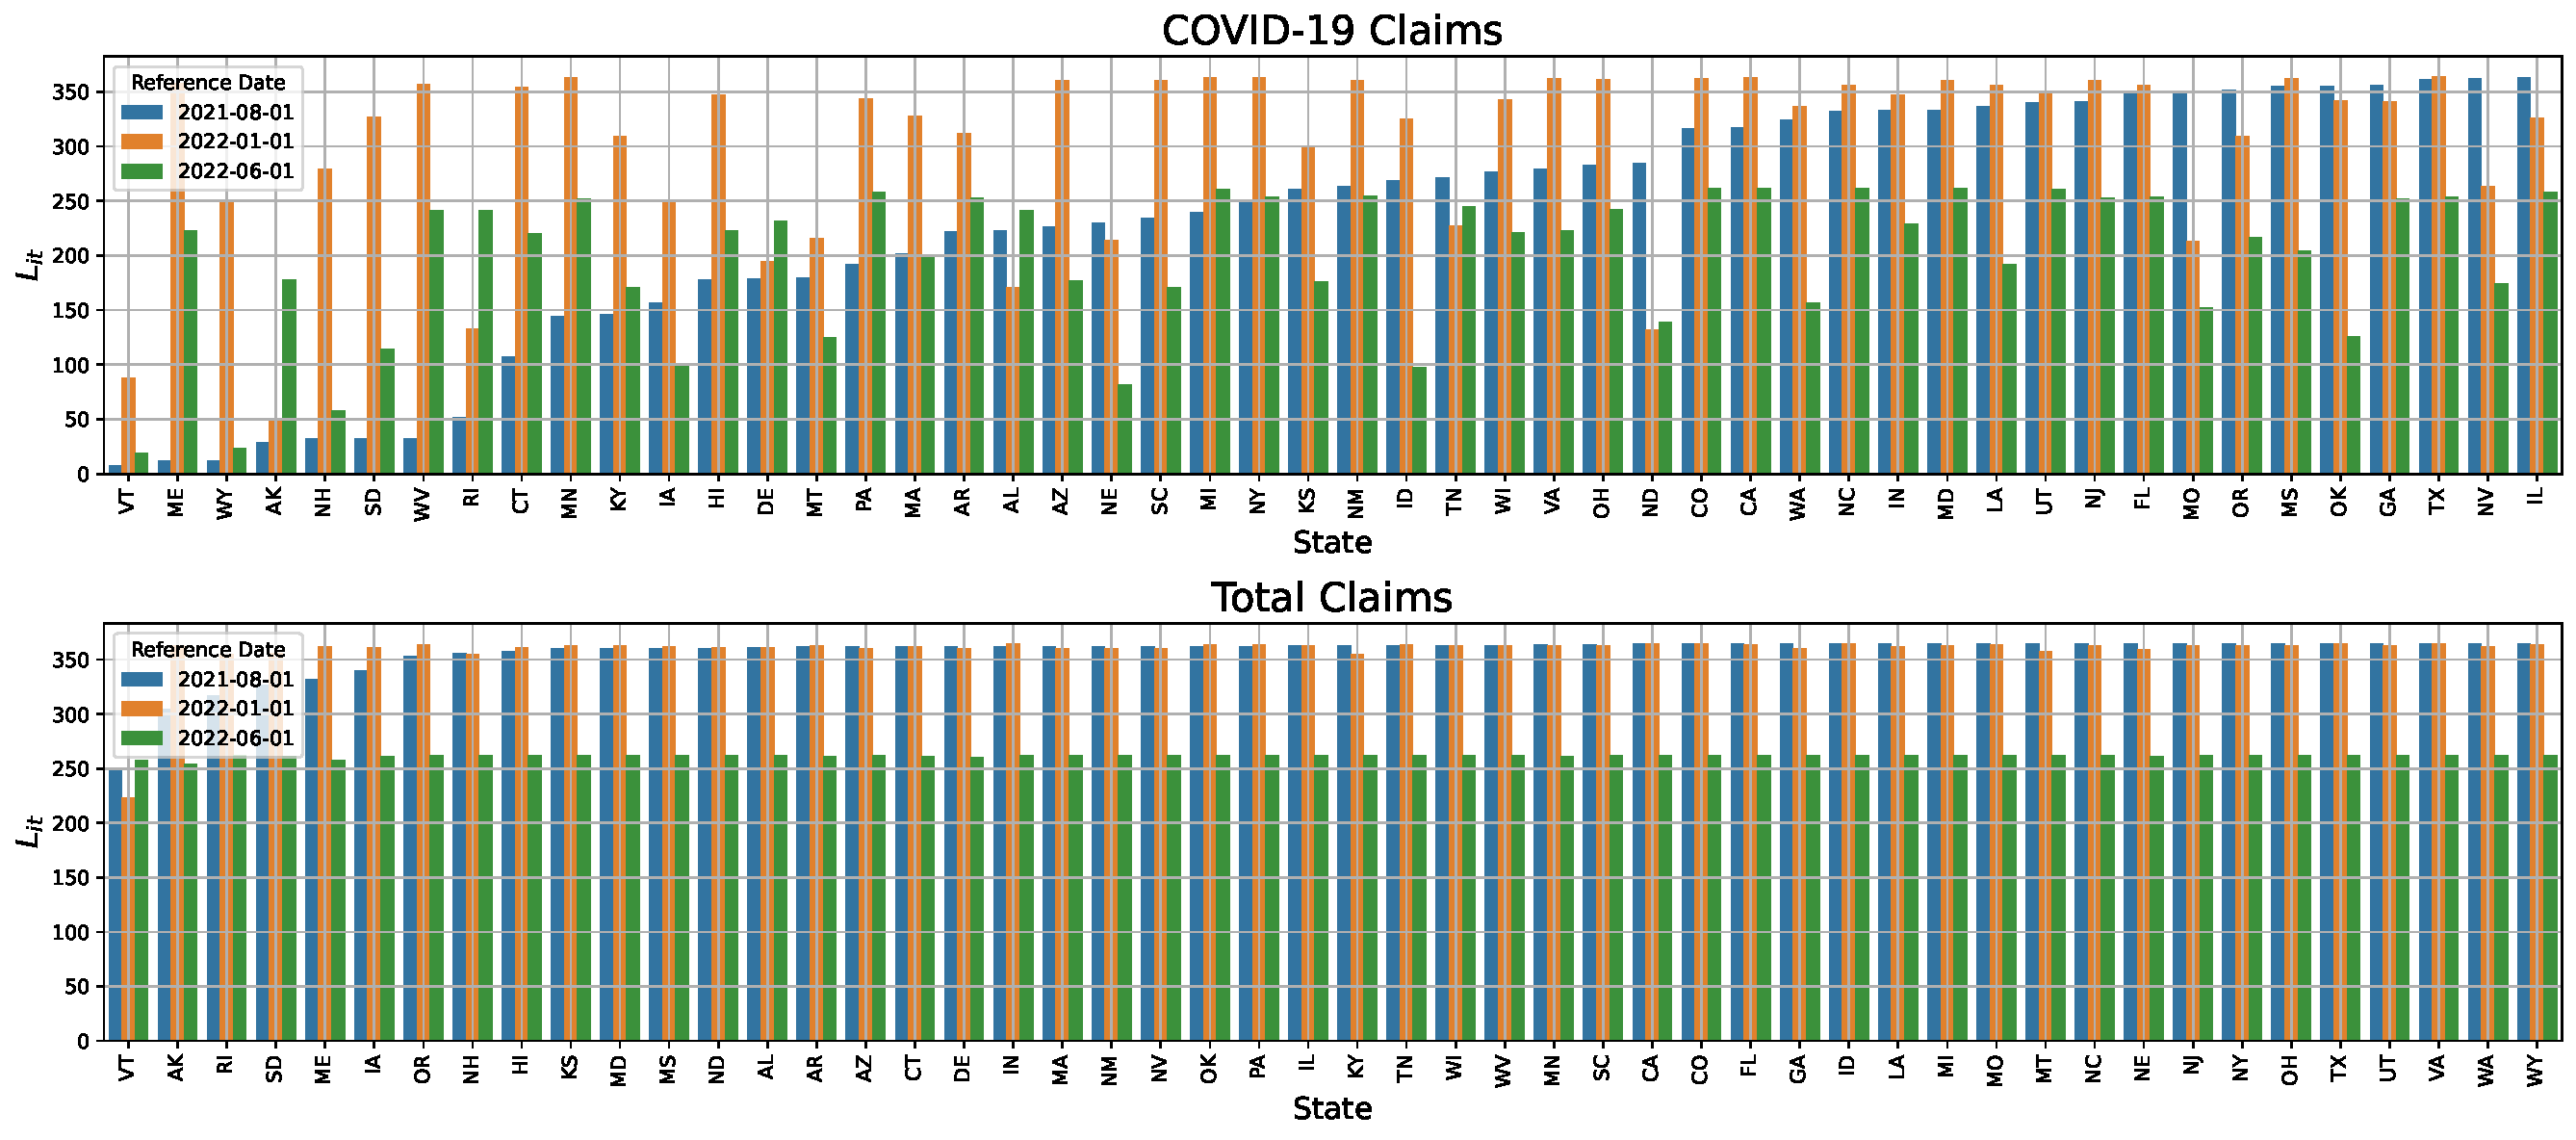
\includegraphics[width=\textwidth]{figs/Lit_examples.pdf}
    \caption{\emph{\textbf{Lag convergence patterns across states.} Top: Comparison of the lags required for convergence across states, shown for a sample of different reference dates based on CHNG outpatient COVID-19 insurance claims. Bottom: Same as the top panel, but based on CHNG outpatient total insurance claims data.}}

\end{figure}


\section{Computational Cost of Training Window Variation for Daily Data}

\begin{table}[h!]
\centering
\resizebox{\textwidth}{!}{%
\begin{tabular}{|c|c|c|c|c|}
\hline
\multicolumn{2}{|c|}{\textbf{Computing Time (s)} (per location per report date)} 
& \multicolumn{3}{c|}{\textbf{Model}} \\
\hline
\makecell{\textbf{Training Window}\\\textbf{(days)}} & \textbf{Data} 
& \makecell{Delphi-RF\\Training\\(once/week or month)} 
& \makecell{Epinowcast} 
& \makecell{NobBS} \\
\hline
\multirow{2}{*}{180} 
& \makecell{Confirmed Cases\\(Daily, State, MA only)} & $6.773 \pm 0.018$   &$406.097\pm 16.190$ &$24.220\pm 0.675$ \\
& \makecell{Insurance Claims\\(Daily, State, All states)} & $23.712\pm 0.029$ &$2386.512 \pm 230.895$ &$96.012 \pm  0.453$ \\
\hline
\multirow{2}{*}{365} 
& \makecell{Confirmed Cases\\(Daily, State, MA only)} & $7.348 \pm 0.024$  &$1289.363\pm 79.974$ &$59.549\pm 1.011$ \\
& \makecell{Insurance Claims\\(Daily, State, All states)} & $37.389\pm 0.042$ &- &$297.092 \pm 1.709$ \\ 
\hline
\end{tabular}

}
\caption{\emph{\textbf{Runtime comparison across methods for daily data at different training windows.}
This table presents the mean and standard error of the mean (SEM) for computing time (in seconds) required by different forecasting methods, applied to daily COVID-19 datasets. Results are reported per reference date and location. Models are trained and used to generate forecasts every 30 days for CHNG insurance claims data and every 7 days for MA-DPH confirmed case data. The comparison is performed under two training window settings (180 and 365 days), with all other configurations held constant to ensure a fair evaluation of runtime differences across methods.}}
\label{tab:full-width}
\end{table}

\clearpage
\section{Complete Set of DelphiRF Revision Forecasts by Reference Date}

Figures S2–S51 present DelphiRF revision forecasts for CHNG-provided insurance claims data at lag 7 across all 50 U.S. states. The model is re-trained every 30 days using training windows of 180 and 365 days, respectively. The format follows that of Figures 5 and 6 in the main text.

\foreach \state in \statepdfs {
  \begin{figure}[H]
    \centering
    \includegraphics[width=0.85\textwidth]{figs/appendix_\state_experiment_result_Insurance_claims_time_series.pdf}
    \caption{\emph{Forecast Accuracy for \MakeUppercase{\state}.}}
    \label{fig:claims-\state}
  \end{figure}
}

\clearpage
\section{Annotated Trend Categories in Target Values Across States}


\begin{figure}[h!]
    \centering
    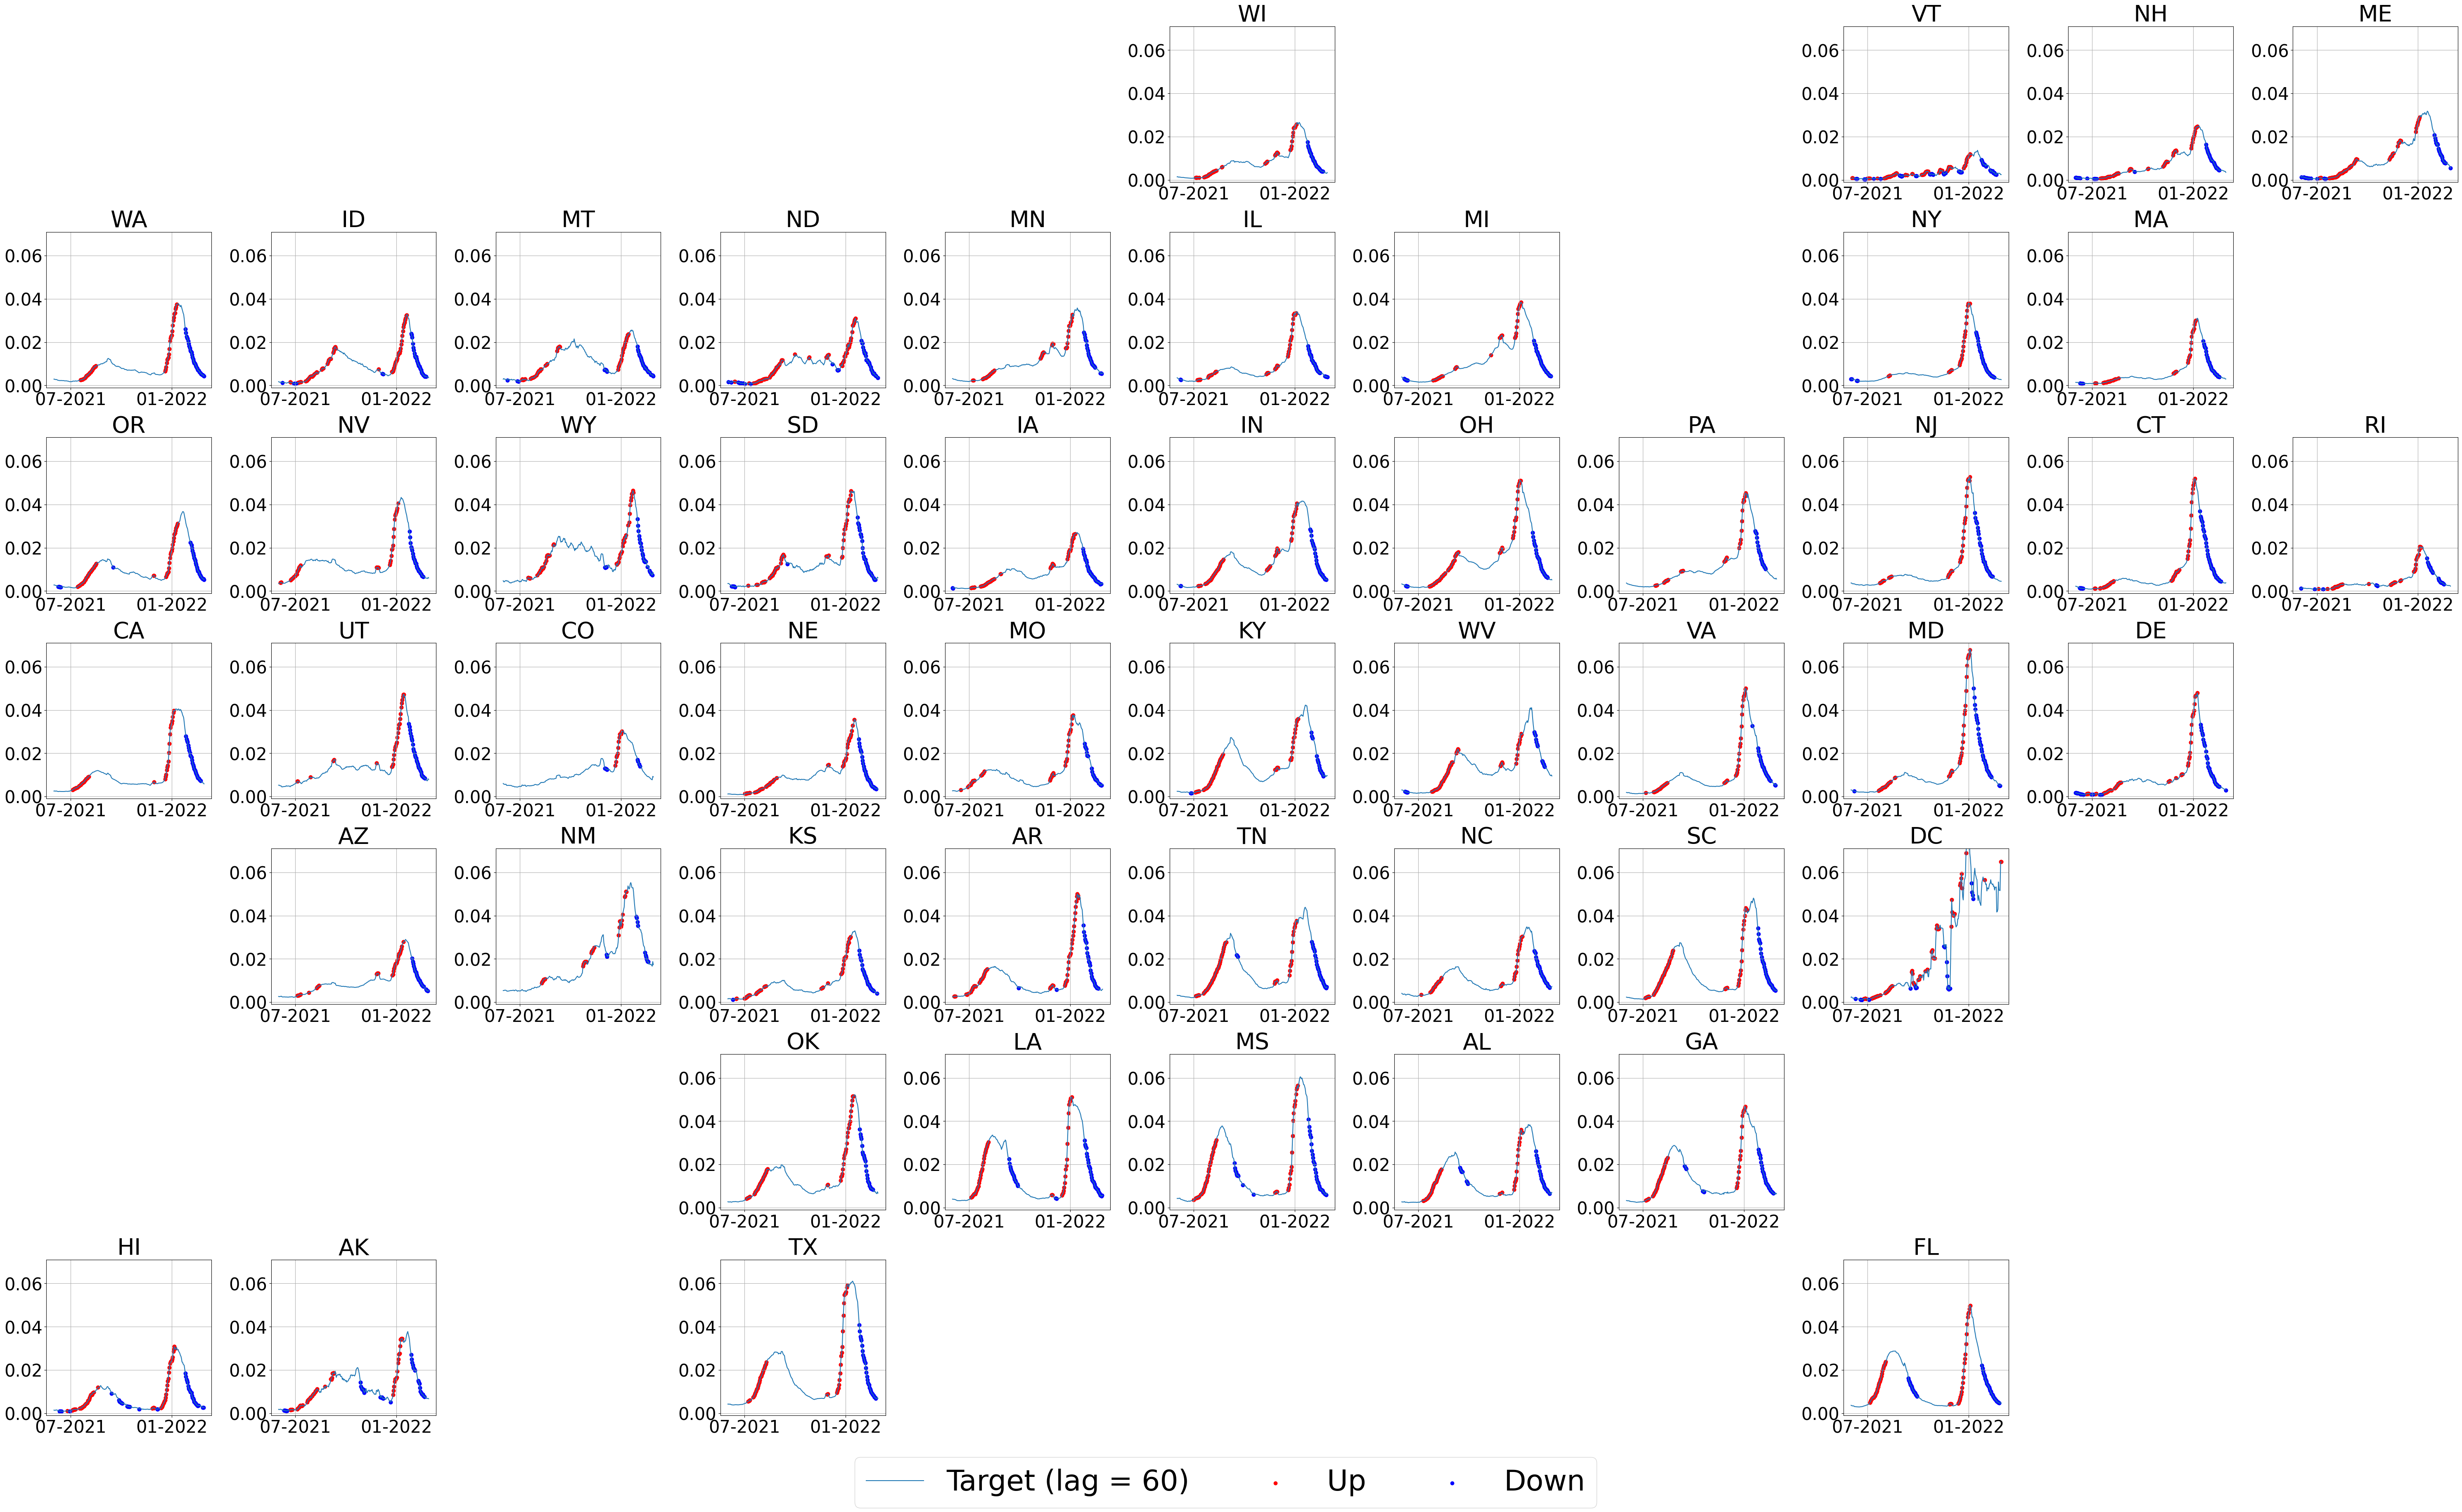
\includegraphics[width=\textwidth]{figs/temporal_annotation_for_states.png}
    \caption{\emph{Temporal Annotation of Trend Categories}}
\end{figure}
